\documentclass{article}

\usepackage[utf8]{inputenc}
\usepackage{enumitem}
\usepackage{latexsym}
\usepackage{amsfonts}
\usepackage{amsmath,amssymb,amsthm}
\usepackage{amsfonts}
\usepackage{parskip}
\usepackage{listings}

\usepackage{tikz}
\usetikzlibrary{arrows, automata, bending, positioning}

\title{Homework 2}
\author{Asier Garcia Ruiz}

\newenvironment{question}[2]
{
    {\large \textbf{Question #1.}}\\
    #2\\\\
}{\newpage}

\begin{document}
\maketitle

\begin{question}{1.1. Nondeterminism}
    {
        (2 points - \textit{Section A}) For any regular language $L$, give a NFA that
        accepts $L_1 = \{axb ~|~$ $x \in L, a, b \in \Sigma^*\}$, i.e. the set of all
        strings that contain a string from $L$ as a substring.
    }
    The new NFA looks as such

    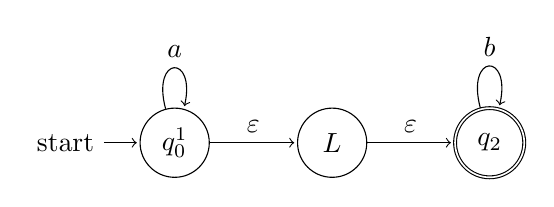
\begin{tikzpicture}[shorten >=1pt,node distance=2cm,on grid,auto]
        \node[state, initial]   (q_0)                       {$q_0^1$};
        \node[state]   (L)    [right of=q_0]                             {$L$};
        \node[state, accepting]   (q_2)  [right of=L]                              {$q_2$};

        \path[->]   (q_0) edge [loop above] node {$a$} ()
        (q_0) edge node {$\varepsilon$} (L)
        (L) edge node {$\varepsilon$} (q_2)
        (q_2) edge [loop above] node {$b$} ()
        ;
    \end{tikzpicture}

    Here, the node $L$ represents the NFA for the regular language $L$. Let this NFA be
    represented as $M_0 = (Q_0, \Sigma_0, \delta_0, q_0^0, F_0)$. Now, we define our new NFA
    $M_1 = (Q_1, \Sigma_1, \delta_1, q_0^1, F_1)$ that recognises $L_1$. We define the
    elemnts of the 5 tuple as follows:
    \begin{align*}
        Q_1      & = \{q_0^1, q_2\} \cup Q_0,                          \\
        \Sigma_1 & = \Sigma_0 \ \text{since $a,b \in \Sigma$},         \\
        \delta_1 & = \begin{cases}
                         \delta_1(q_0, a) = q_0^1,                         \\
                         \delta_1(q_0^1, \varepsilon) = q_0^0,             \\
                         \delta_1(q_2, b) = q_2,                           \\
                         \delta_1(q, \epsilon) = q_2   & q \in F_0,        \\
                         \delta_0(q, a) = \delta(q, a) & \text{otherwise,}
                     \end{cases} \\
        q_0^1    & = q_0^1 \ \text{as in the figure},                  \\
        F_1      & = \{q_2\}
    \end{align*}
    This NFA $M_1$ accepts $L_1$.
\end{question}

\begin{question}{1.2. Nondeterminism}
    {
        (2 points - \textit{Both}) For any regular language $L$, prove that $L' = $
        $\{xay\ |\ xy \in L, a \in \Sigma, x, y \in \Sigma^*\}$ is regular, i.e. the set of
        all strings from which deleting exactly one character gives a string from $L$. For
        example, if $L$ were binary palindromes (words that are the same when reversed),
        some words in $L'$ would include 1001\textcolor{red}{0}, \textcolor{red}{1}00,
        1110001\textcolor{red}{0}11, since deleting the red character from each string
        produces a palindrome.
    }
    Let $M = (Q, \Sigma, \delta, q_0, F)$ be an NFA that recognises $L$ and
    let $M' = (Q', \Sigma', \delta', q_0', F')$ be an NFA that accepts $L'$ and
    Let $Q_{int}$ be a set of intermediate states for every state in
    $Q$, and let $Q_2, Q_3$ be two copies $Q$. We denote $q_i^j$ as the $i$th state
    in $Q_j$.
    We will define the elements of $M'$ as follows:
    \begin{align*}
        Q'            & = Q \cup Q_{int} \cup Q_2 \cup Q_3,                  \\
        \Sigma'       & = \Sigma,                                            \\
        \delta'(q, a) & = \begin{cases}
                              q^1_i & \text{if } q \in Q_2,                      \\
                              q^3_i & \text{if } q \in Q_{int}, a = \varepsilon, \\
                          \end{cases} \\
        q_0'          & = q_0^1,                                             \\
        F'            & = F                                                  \\
    \end{align*}

    We have constructed $M'$, an NFA that recognises $L'$. Thus, $L'$ is regular.

\end{question}

\begin{question}
    {2.1. Regular Expressions}
    {(2 points) Give a regular expression for each of the following languages:
        \begin{itemize}
            \item The set of all strings with an even number of 1's.
            \item The set of all even length strings with at most two 0's
        \end{itemize}
        \ }
    \begin{itemize}
        \item $(0 \cup (10^*1))^*$
        \item Let \[R_1 = (11)^*\]
              be the expression of even length strings with no zeros. Then,
              \[R_2 = (11)^*((01)\cup(01)(11)^*)\]
              is the expression of even length string with exactly 1 zero.
              Finally,
              \begin{align*}
                  R_3 & =(11)^*0(11)^*0(11)^*       \\
                      & \cup (11)^*01(11)^*01(11)^* \\
                      & \cup 1(11)^*01(11)^*        \\
                      & \cup 1(11)^*01(11)^*0(11)^*
              \end{align*}
              is the expression for all strings of even length with exactly 2 zeros.
              Combining these we get our answer
              \[R = R_1 \cup R_2 \cup R_3\]
    \end{itemize}
\end{question}

\begin{question}
    {2.2. Regular Expressions}
    {(2 points) Give an equivalent NFA for the following regular expression:

        $((01 \cup 10^*1 \cup 10)1)^*(00)^*$}

    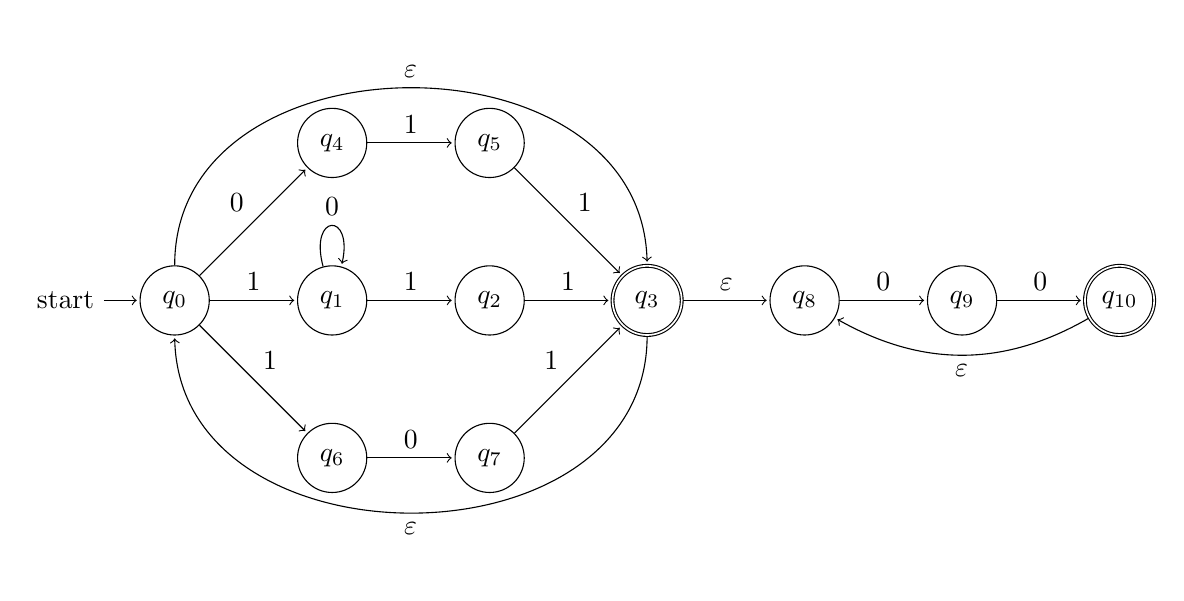
\begin{tikzpicture}[shorten >=1pt,node distance=2cm,on grid,auto]
        \node[state, initial]       (q_0)                                  {$q_0$};
        \node[state]                (q_1)    [right of=q_0]                {$q_1$};
        \node[state]                (q_2)    [right of=q_1]                {$q_2$};
        \node[state, accepting]     (q_3)    [right of=q_2]                {$q_3$};

        \node[state]                (q_4)    [above of=q_1]                {$q_4$};
        \node[state]                (q_5)    [right of=q_4]                {$q_5$};

        \node[state]                (q_6)    [below of=q_1]                {$q_6$};
        \node[state]                (q_7)    [right of=q_6]                {$q_7$};

        \node[state]                (q_8)    [right of=q_3]                {$q_8$};
        \node[state]                (q_9)    [right of=q_8]                {$q_9$};
        \node[state, accepting]     (q_10)   [right of=q_9]               {$q_{10}$};

        \path[->]   (q_0) edge node {1} (q_1)
        edge node {1} (q_6)
        edge node {0} (q_4)
        edge [bend left=90, distance=3cm] node {$\varepsilon$} (q_3)
        (q_1) edge [loop above] node {0} ()
        edge node {1} (q_2)
        (q_2) edge node {1} (q_3)
        (q_3) edge node {$\varepsilon$} (q_8)
        edge [bend left=90, distance=3cm] node {$\varepsilon$} (q_0)
        (q_4) edge node {1} (q_5)
        (q_5) edge node {1} (q_3)
        (q_6) edge node {0} (q_7)
        (q_7) edge node {1} (q_3)
        (q_8) edge node {0} (q_9)
        (q_9) edge node {0} (q_10)
        (q_10) edge [bend left=30] node {$\varepsilon$} (q_8)
        ;
    \end{tikzpicture}
\end{question}

\begin{question}
    {3. Pumping Lemma}
    {(\textit{Section A}) Prove that $L_1 = \{a^ib^j\ |\ |i-j|$ is prime$\}$ is not
        regular.}
    Assume, for the sake of contradiction, that $L_1$ is regular and let $p$ be the
    pumping length. Now, let $s = 0^{p+2}1^j$ such that $|p + 2 - j|$ is prime. We have
    that $s \in L_1$ so by the pumping lemma we can rewrite $s = xyz$. We also have
    that $|xy| \leq p$, therefore $y$ consists of only zeros, let $|y| = k$.
    Now, consider $xyyyz = 1^{p+2}1^k1^kb^p \in L_1$, this implies
    $|p + 2 + k + k - p| = |2 + 2k|$ is prime. This is clearly a contradiction
    as $|2 + 2k|$ is divisible by 2. Therefore, $L_1$ is not regular.
\end{question}

\begin{question}
    {4. Pumping Lemma Adjacent}
    {A \emph{minimal} DFA $D$ for a language $L$ is a $DFA$ such that any DFA for
        $L$ has at least as many states as $D$.  Complete the steps below to prove the
        following claim:

        \emph{Claim:} For any positive integer $n \geq 3$, there is a language whose
        minimal DFA contains $n$ states.

        \emph{Proof:} For some $k \in \mathbb{Z}$, let $L_k = \{a^k\}$, a set with one
        element. Now, suppose $D$ is a minimal DFA for $L_k$. You will prove that $D$ has
        at least $k+2$ states.  Let $\{q_i\}_{i=0}^k = q_0, ..., q_k$ be the sequence of
        states (not necessarily distinct!) that $D$ follows when reading $a^k$.

        (1 points) Explain why $\{q_i\}_{i=0}^k$ cannot contain any repeated states
        (hint: the proof of the pumping lemma), and conclude that $D$ has at least $k+1$
        states.

        (1 point) Now consider the state that $D$ ends in upon reading the string
        $a^{k+1}$, and argue that $D$ must have at least $k+2$ states.

        (1 point) Demonstrate that $D$ has exactly $k+2$ states by giving an explicit
        construction of $D$.

        (1 point) Complete the conclusion of this proof: ``Therefore, we have given a
        constructive proof of the original claim. For any $n \in \mathbb{Z}, n \geq 3$, the
        language \_\_\_\_\_\_\_\_\_\_ has a minimal DFA with $n$ states."}

    1.\\
    We have that $|\{q_i\}_{i=0}^k| = k + 1$. Therefore, by the Pigeonhole principle,
    we need at least $k + 1$ states in $D$ to avoid repeated states. This cannot happen
    since it would imply that for the same input the DFA would have two possible
    transitions.

    2.\\
    We can show this easily by induction. If $k = 0$ then we need one state
    (a single, starting/accepting state). Now, we have shown that for the string
    $a^k$ we need $k + 1$ states. If we now make this $a^{k + 1} = a^ka$ we
    need exactly one more state (i.e. $k + 2$ states). Therefore,
    given $a^{k+1}$ we need $k + 2$ states.

    3.\\
    We will construct a DFA $M = (Q, \Sigma, \delta, q_0, F)$ that recognises $L_k$
    We will define the elements of the five tuple as follows
    \begin{align*}
        Q              & = \{q_i\}_{i=0}^{k+2},                          \\
        \Sigma         & = \Sigma_L \text{(i.e. the alphabet of $L_k$)}, \\
        \delta(q_i, x) & = \begin{cases}
                               q_{i+1}   & \text{if } x = a, i \neq k + 2, \\
                               q_{k + 2} & \text{otherwise}
                           \end{cases},   \\
        q_0            & = q_0,                                          \\
        F              & = \{q_{k+1}\}
    \end{align*}

    4.\\
    (1 point) Complete the conclusion of this proof: ``Therefore, we have given a
    constructive proof of the original claim. For any $n \in \mathbb{Z}, n \geq 3$, the
    language $L_n = \{a^{n-2}\}$ has a minimal DFA with $n$ states."

\end{question}

\end{document}